% !TeX encoding = UTF-8
\documentclass[aspectratio=169]{beamer}
\useoutertheme[progressbar=frametitle]{metropolis}
\useinnertheme{metropolis}
\definecolor{nabgray}{rgb}{0.6,0.59,0.61}
\usecolortheme[named=nabgray]{structure}

\usepackage{tikz}
\usepackage[utf8]{inputenc}
\usepackage[spanish]{babel}
\usepackage{fontspec}
\setmonofont{JetBrains Mono}
\setmainfont{Roboto}
\setsansfont{Roboto}

\usepackage{smartdiagram}
\usepackage{qtree}
\usepackage{verbatim}
\usepackage{svg}
\usepackage{graphicx}
\usepackage{color}

\definecolor{lightgray}{rgb}{0.95, 0.95, 0.95}
\definecolor{darkgray}{rgb}{0.4, 0.4, 0.4}
%\definecolor{purple}{rgb}{0.65, 0.12, 0.82}
\definecolor{editorGray}{rgb}{0.95, 0.95, 0.95}
\definecolor{editorOcher}{rgb}{1, 0.5, 0} % #FF7F00 -> rgb(239, 169, 0)
\definecolor{editorGreen}{rgb}{0, 0.5, 0} % #007C00 -> rgb(0, 124, 0)
\definecolor{orange}{rgb}{1,0.45,0.13}
\definecolor{olive}{rgb}{0.17,0.59,0.20}
\definecolor{brown}{rgb}{0.69,0.31,0.31}
\definecolor{purple}{rgb}{0.38,0.18,0.81}
\definecolor{lightblue}{rgb}{0.1,0.57,0.7}
\definecolor{lightred}{rgb}{1,0.4,0.5}
\usepackage{upquote}
\usepackage{listings}
\lstset{language=java,
	basicstyle=\footnotesize\ttfamily,
	keywordstyle=\footnotesize\color{blue}\ttfamily,
	escapeinside={<@}{@>}
}


\usebackgroundtemplate%
{%
	
\includegraphics[width=\paperwidth]{Images/Contenido}%
}


\title{GraalVM: Aplicaciones nativas AOT para los lenguajes de la JVM}
\author{Víctor Orozco}
\institute{Nabenik}
\date{\today}

\begin{document}





{
    \usebackgroundtemplate{
\includegraphics[width=\paperwidth]{Images/portada}}
    \setbeamercolor{frametitle}{fg=red}
    \usebeamercolor[fg]{normal text}
    \frame{\titlepage}
}


\begin{frame}{GraalVM}
¿Que es GraalVM
	\begin{itemize}
		\item Maquina virtual políglota por Oracle Labs
		\item JVM Langs, Truffle, LLVM
        \item Escrita en Java
        \item Open Source y Enterprise Edition
	\end{itemize}
\end{frame}


\begin{frame}{}
\begin{figure}
	\centering
	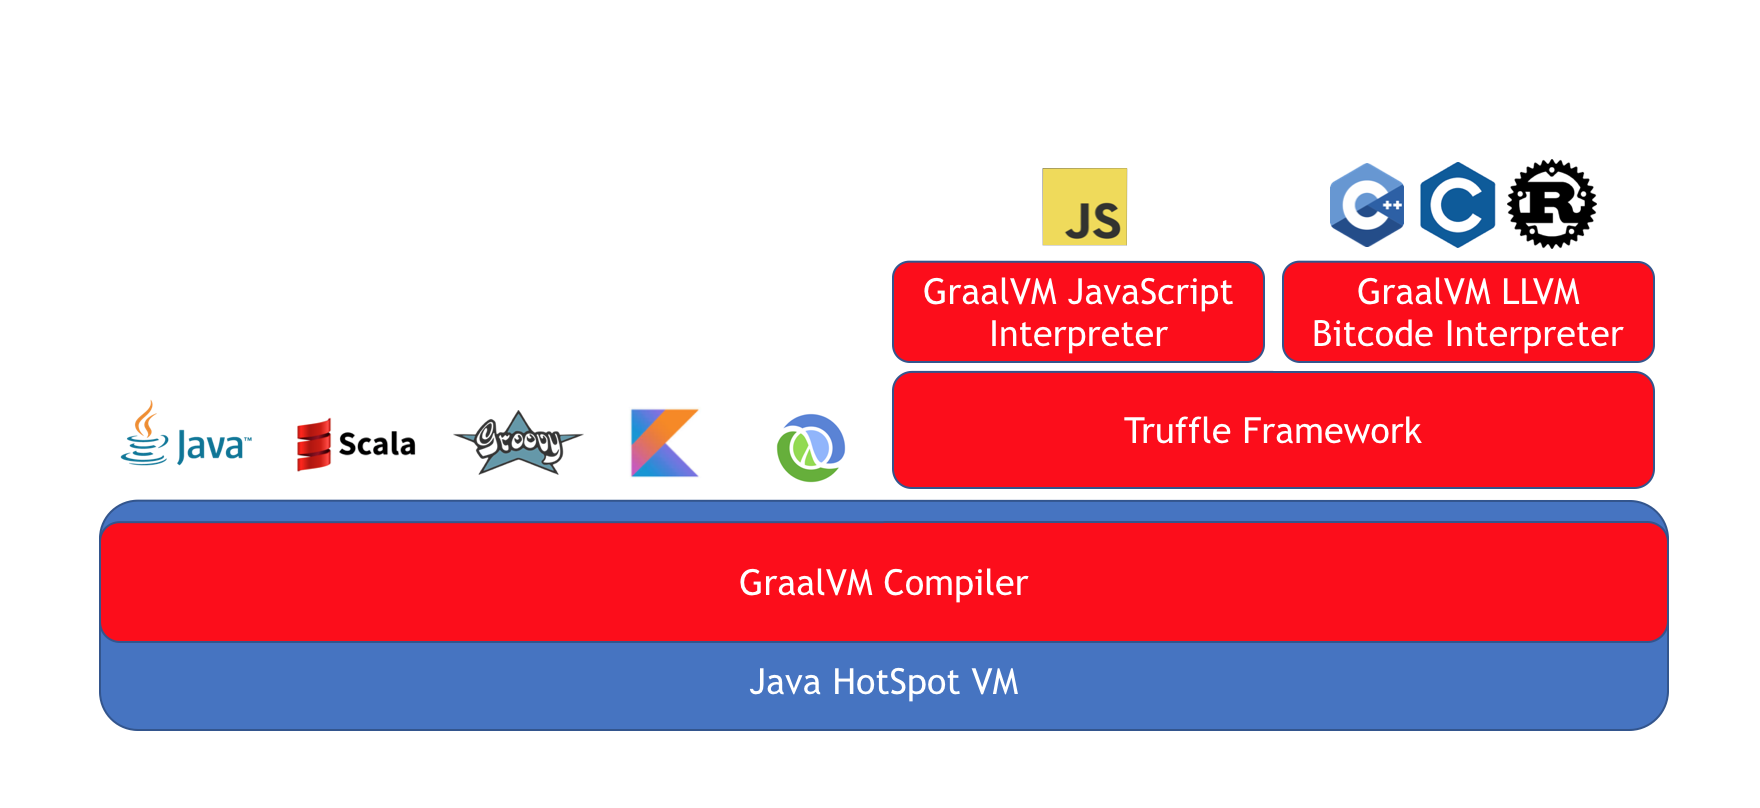
\includegraphics[width=\linewidth]{Images/graalvm}
	\caption{GraalVM Overview}
	\label{fig:graalvm}
\end{figure}

\end{frame}

\begin{frame}{GraalVM}
	
	\begin{columns}[T] % contents are top vertically aligned
		
		\begin{column}[T]{4cm} % alternative top-align that's better for graphics
			Puntos a resaltar
		\begin{enumerate}
			\item TCK'd JDK
			\item Compilador JIT
			\item \textbf{Java Native Image}
			\item Polyglot VM
		\end{enumerate}
		\end{column}
		\begin{column}[T]{6cm} % each column can also be its own environment
			\begin{figure}
				\centering
				
\includegraphics[width=\linewidth]{Images/graalvmlogo}

			\end{figure}
			
		\end{column}
	\end{columns}
	

\end{frame}


\begin{frame}{TCK'd JDK}

	\begin{figure}
		\centering
		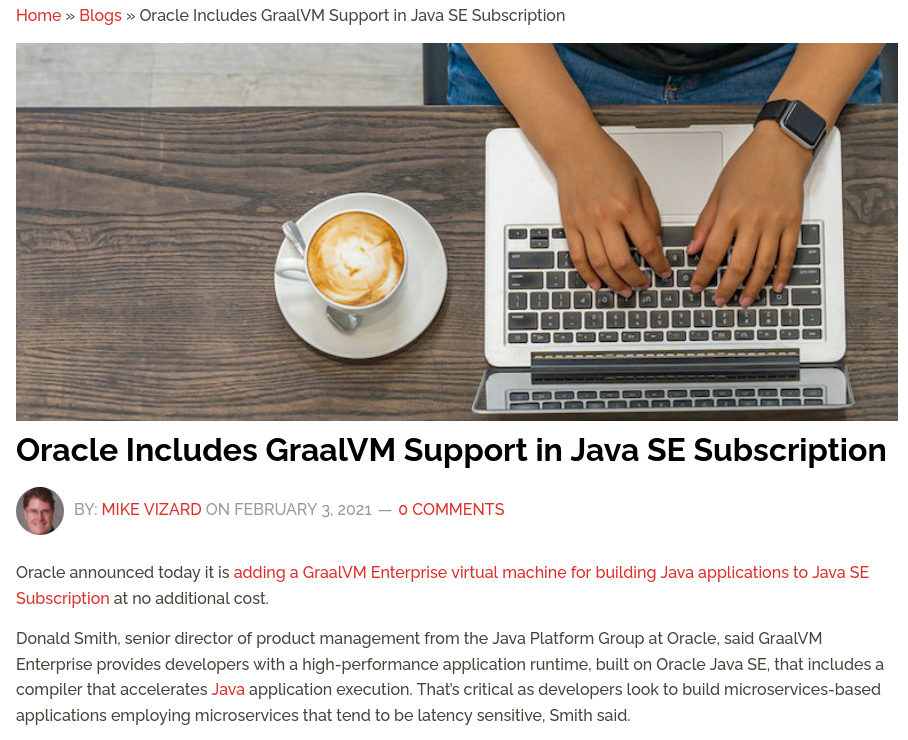
\includegraphics[width=0.55\linewidth]{Images/tckjdk}
	\end{figure}
{\tiny 
https://blogs.oracle.com/java/ways-graalvme-adds-value-to-java-se-subscription
}
\end{frame}


\begin{frame}{GraalVM como JIT}
	\begin{figure}
		\centering
		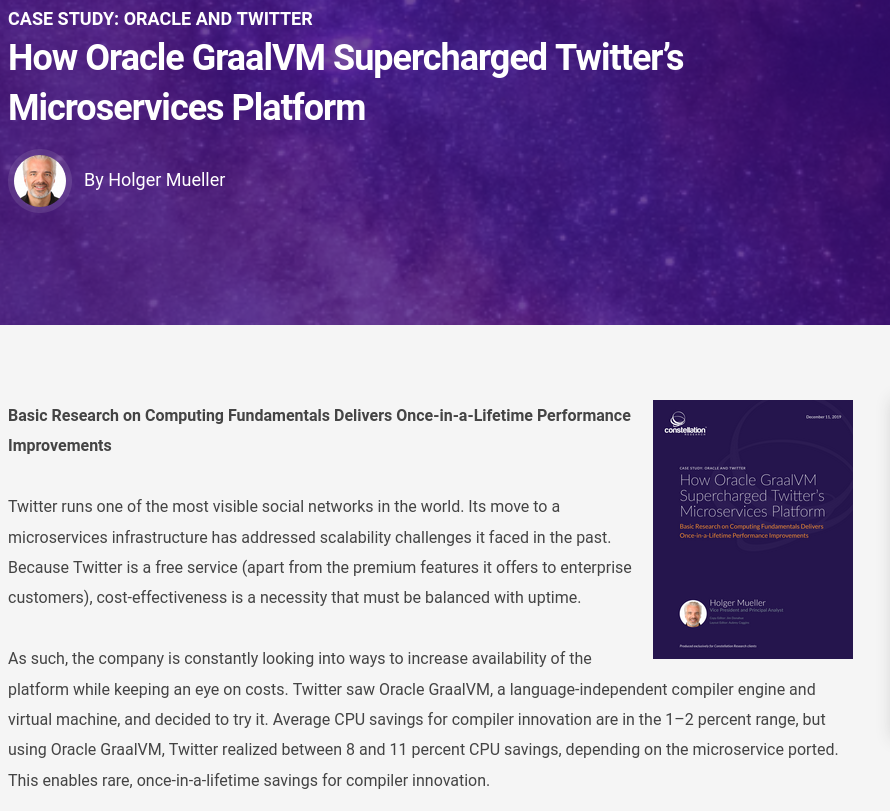
\includegraphics[width=0.5\linewidth]{Images/twittergraalvm}
	\end{figure}
{\tiny 
https://www.constellationr.com/research/how-oracle-graalvm-supercharged-twitter-s-microservices-platform
}
\end{frame}

{
	\usebackgroundtemplate{
\includegraphics[width=\paperwidth]{Images/separador}}
	\setbeamercolor{normal text}{fg=white}
	\setbeamercolor{frametitle}{fg=red}
	\usebeamercolor[fg]{normal text}
	\section{Imagenes nativas}
}



\begin{frame}{Java Virtual Machine}
	
	\begin{itemize}
		\item Thread scheduling, gestión de memoria
		\item JVM se desarrolló en los 90's y 2000 como un entorno con compilación JIT (C2)
		\item Peak performance 
		\item Detección de hotspots
	\end{itemize}
	
\end{frame}



\begin{frame}{}
	\begin{figure}
		\centering
		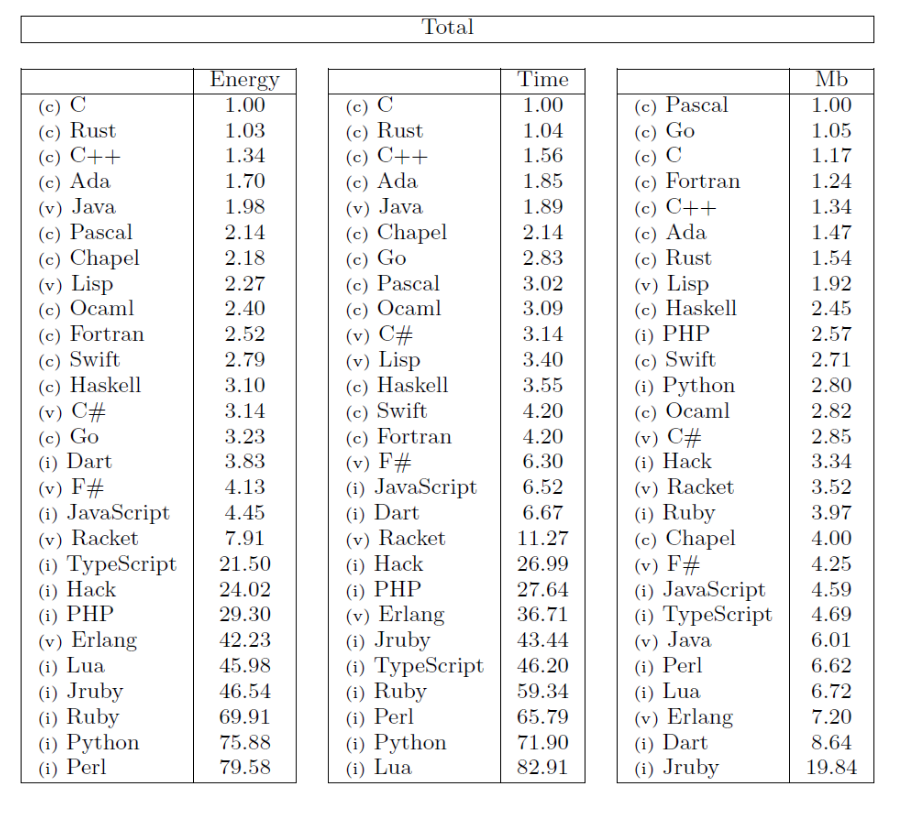
\includegraphics[width=0.6\linewidth]{Images/energy.png}
	\end{figure}
{\tiny https://greenlab.di.uminho.pt/wp-content/uploads/2017/10/sleFinal.pdf}
\end{frame}

\begin{frame}{GraalVM Native}
	\begin{figure}
		\centering
		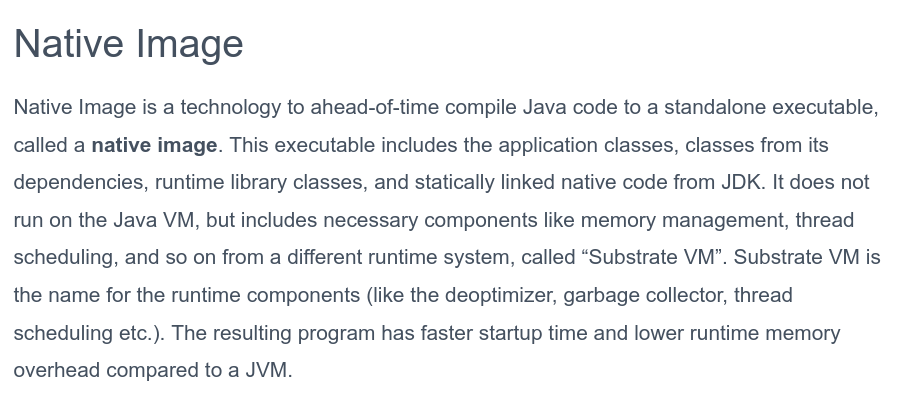
\includegraphics[width=\linewidth]{Images/nativeimagedefinition.png}
	\end{figure}
{\tiny https://www.graalvm.org/reference-manual/native-image/}
\end{frame}

\begin{frame}{GraalVM Native}
	
	\begin{block}{Compilación AOT - Wikipedia}
		En informática, Compilación anticipada es el acto de compilar un lenguaje de programación de alto nivel como C o C++, o un lenguaje intermedio como Java bytecode o el Common Intermediate Language de .NET, a un \textbf{código de máquina nativo} con la intención de ejecutar el archivo binario resultante nativamente
	\end{block}
	
\end{frame}


\begin{frame}{GraalVM Native}
	
	\begin{block}{Static Linking - Indiana University}
		El enlace estático es el resultado de que el enlazador copia todas las rutinas de la biblioteca utilizadas en el programa en la imagen ejecutable. Esto puede requerir más espacio en disco y memoria que la vinculación dinámica, pero es más rápido y más portátil, ya que no requiere la presencia de la biblioteca en el sistema donde se ejecuta.
	\end{block}
	
\end{frame}


\begin{frame}{GraalVM Native}
	
	\begin{exampleblock}{GraalVM Native}
	GraalVM Native es una tecnología de \textbf{compilación AOT de bytecode Java}. Permite crear un \textbf{ejecutable con static linking} que incluye clases, bibliotecas y los modulos necesarios del JDK junto a SubstrateVM
	\end{exampleblock}
	
\end{frame}




\begin{frame}{Algunas otras implementaciones Bytecode AOT}
	\begin{itemize}
		\item ExcelsiorJET
		\item GNU Compiler for Java
		\item ART (Android)
		\item \textbf{IBM OpenJ9}
	\end{itemize}

\end{frame}




\begin{frame}{GraalVM Native}
	\begin{figure}
		\centering
		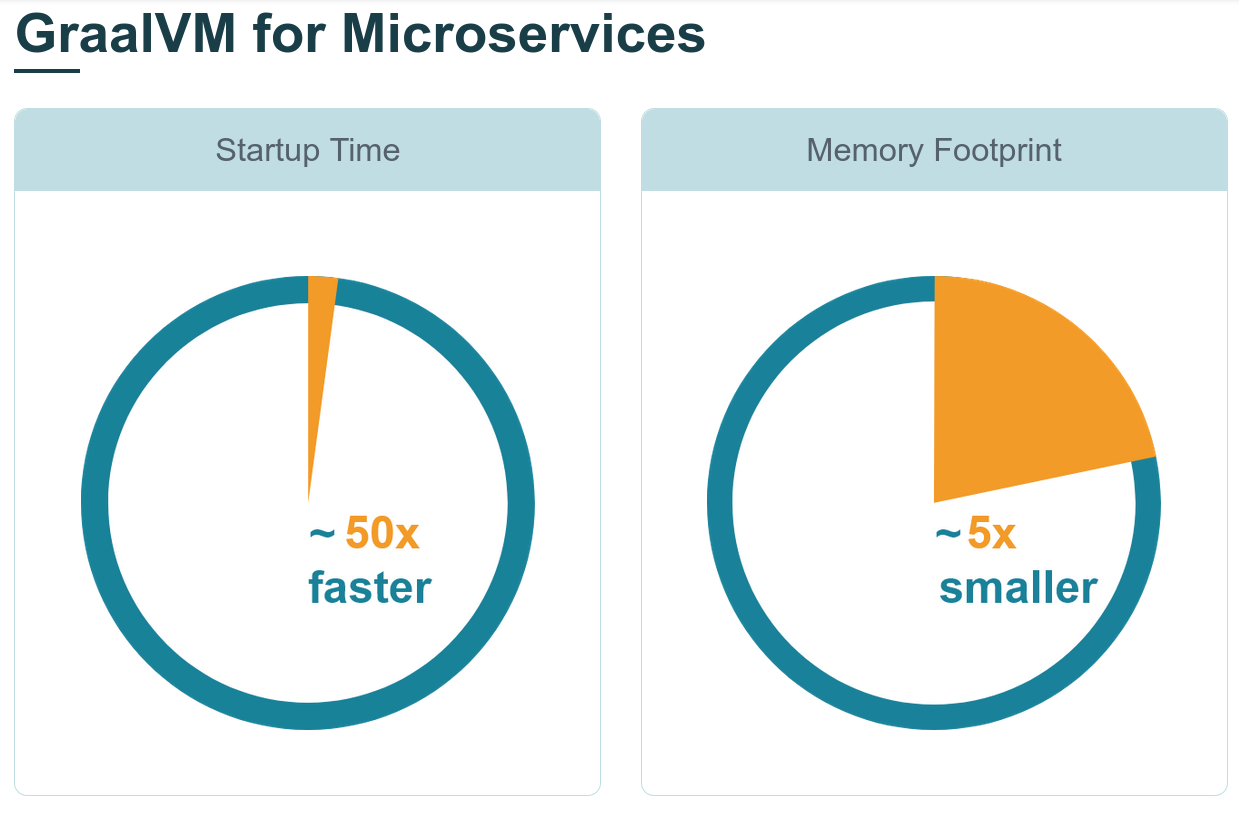
\includegraphics[width=0.7\linewidth]{Images/ventajasnative}
	\end{figure}
\end{frame}

\begin{frame}{GraalVM Native}
	\begin{figure}
		\centering
		
\includegraphics[width=\linewidth]{Images/implementacionesnative}
	\end{figure}
\end{frame}

\begin{frame}{Demo 1}
	\begin{itemize}
		\item Proyecto Java 11
		\item Maven
		\item El hola mundo más rapido del oeste
	\end{itemize}
\end{frame}

\begin{frame}{Demo 2}
	\begin{itemize}
		\item kservice-a: Kotlin 1.4, MicroProfile, Oracle Helidon
		\item jservice-b: Java 11, MicroProfile, Red Hat Quarkus
		\item Kubernetes
		\item Docker
	\end{itemize}
\end{frame}



{
	\usebackgroundtemplate{
\includegraphics[width=\paperwidth]{Images/separador}}
	\setbeamercolor{normal text}{fg=white}
	\setbeamercolor{frametitle}{fg=red}
	\usebeamercolor[fg]{normal text}
	\section{Consideraciones finales}
}


\begin{frame}{Consideraciones finales}
	
	\begin{columns}[T] % contents are top vertically aligned
		
		\begin{column}[T]{4cm} % alternative top-align that's better for graphics
			\begin{exampleblock}{Ventajas}
				\begin{itemize}
					\item Compilación AOT
					\item Menor consumo de memoria
					\item Menor tiempo de arranque
					\item Casos útiles: CLI, Aplicaciones de escritorio, Serverless, K8S
				\end{itemize}
			\end{exampleblock}
		\end{column}
		\begin{column}[T]{6cm} % each column can also be its own environment
			\begin{alertblock}{Desventajas}
				\begin{itemize}
					\item Menor desempeño a largo plazo
					\item Reflection, dynamic proxies, invoke, bytecode generation
					\item Muchos frameworks y bibliotecas nunca serán compatibles
					\item Un buen servidor CI/CD
					\item A veces threads > procesos (Vert.x)
				\end{itemize}
			\end{alertblock}
		\end{column}
	\end{columns}
\end{frame}


\begin{frame}{Threads vs procesos}
	\begin{figure}
		\centering
		
\includegraphics[width=\linewidth]{Images/rank0}
	\end{figure}
	
	\begin{figure}
		\centering
		
\includegraphics[width=\linewidth]{Images/rank1}
	\end{figure}
	
	\begin{figure}
		\centering
		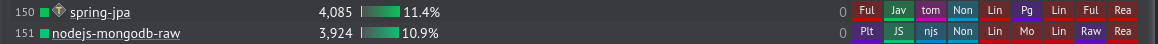
\includegraphics[width=\linewidth]{Images/rank2}
	\end{figure}
{\tiny https://www.techempower.com/benchmarks/\#section=data-r20}
\end{frame}


\begin{frame}{}
	\begin{figure}
		\centering
		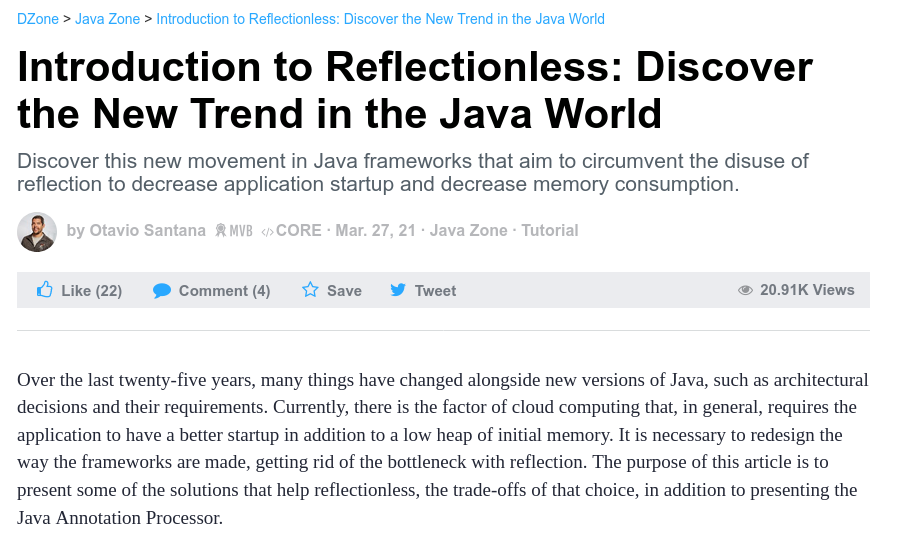
\includegraphics[width=0.8\linewidth]{Images/otavio}
	\end{figure}
{\tiny https://dzone.com/articles/introduction-to-reflectionless-know-what-the-new-t}
\end{frame}

\begin{frame}{Víctor Orozco}
    \begin{columns}[T] % contents are top vertically aligned

        \begin{column}[T]{4cm} % alternative top-align that's better for graphics
            \begin{figure}
                \centering
                
\includegraphics[width=\linewidth]{Images/logos}
            \end{figure}
        \end{column}
        \begin{column}[T]{6cm} % each column can also be its own environment
            \begin{itemize}
                \item vorozco@nabenik.com
                \item \href{https://twitter.com/tuxtor}{@tuxtor}
                \item \href{http://vorozco.com}{http://vorozco.com}
                \item \href{http://tuxtor.shekalug.org}{http://tuxtor.shekalug.org}
            \end{itemize}
            \begin{center}
                
\includegraphics[width=0.1\linewidth]{Images/cclogo}
                \\
                This work is licensed under Creative Commons Attribution-NonCommercial-ShareAlike 3.0 Guatemala (CC BY-NC-SA 3.0 GT).
            \end{center}
        \end{column}
    \end{columns}
\end{frame}



\end{document}
